\documentclass[border=10pt]{standalone}
\usepackage{tikz}
\usetikzlibrary{arrows.meta, shapes, calc}

\begin{document}
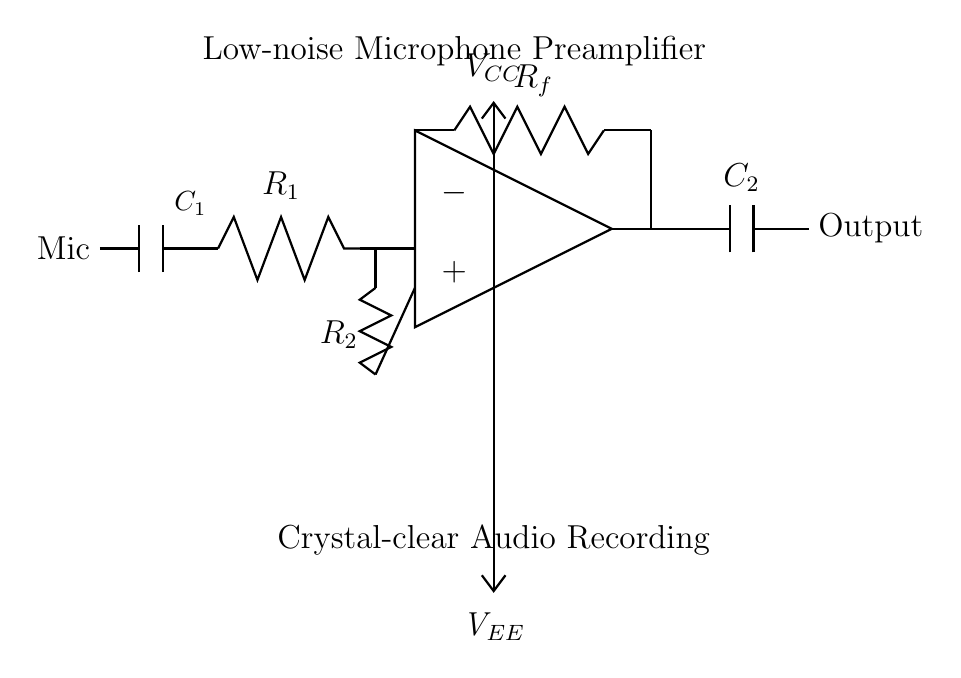
\begin{tikzpicture}[
    >=Stealth,
    resistor/.style={draw, rectangle, minimum width=1cm, minimum height=0.3cm, 
                     path picture={\draw[line width=0.8pt] 
                     (path picture bounding box.west) -- ++(0.1,0) -- ++(0.1,0.15) -- ++(0.15,-0.3) -- ++(0.15,0.3) -- ++(0.15,-0.3) -- ++(0.15,0.3) -- ++(0.1,-0.15) -- ++(0.1,0);}},
    capacitor/.style={draw, line width=0.8pt},
    font=\large
]

% Title
\node at (5, 5.5) {Low-noise Microphone Preamplifier};

% Input capacitor
\draw[line width=0.8pt] (0.5, 3) -- (1, 3);
\draw[line width=0.8pt] (1, 2.7) -- (1, 3.3);
\draw[line width=0.8pt] (1.3, 2.7) -- (1.3, 3.3);
\draw[line width=0.8pt] (1.3, 3) -- (1.8, 3);

% Mic label
\node[left] at (0.5, 3) {Mic};

% R1 resistor
\draw[line width=0.8pt] (1.8, 3) -- (2, 3);
\draw[line width=0.8pt] (2, 3) -- (2.2, 3.4) -- (2.5, 2.6) -- (2.8, 3.4) -- (3.1, 2.6) -- (3.4, 3.4) -- (3.6, 3) -- (3.8, 3);
\node[above] at (2.8, 3.5) {$R_1$};

% Connection to op-amp inverting input
\draw[line width=0.8pt] (3.8, 3) -- (4.5, 3);
\draw[line width=0.8pt] (4.5, 3) -- (4.5, 3.5);

% Op-amp
\draw[line width=0.8pt, fill=white] (4.5, 2) -- (4.5, 4.5) -- (7, 3.25) -- cycle;
\node at (5, 3.7) {$-$};
\node at (5, 2.7) {$+$};

% R2 resistor (between summing node and non-inverting input)
\draw[line width=0.8pt] (4.5, 3) -- (4.0, 3) -- (4.0, 2.5);
\draw[line width=0.8pt] (4.0, 2.5) -- (3.8, 2.35) -- (4.2, 2.15) -- (3.8, 1.95) -- (4.2, 1.75) -- (3.8, 1.55) -- (4.0, 1.4);
\draw[line width=0.8pt] (4.0, 1.4) -- (4.5, 2.5);
\node[left] at (3.9, 1.9) {$R_2$};

% Rf feedback resistor
\draw[line width=0.8pt] (4.5, 3.5) -- (4.5, 4.5);
\draw[line width=0.8pt] (4.5, 4.5) -- (5, 4.5);
\draw[line width=0.8pt] (5, 4.5) -- (5.2, 4.8) -- (5.5, 4.2) -- (5.8, 4.8) -- (6.1, 4.2) -- (6.4, 4.8) -- (6.7, 4.2) -- (6.9, 4.5);
\draw[line width=0.8pt] (6.9, 4.5) -- (7.5, 4.5);
\draw[line width=0.8pt] (7.5, 4.5) -- (7.5, 3.25);
\node[above] at (6, 4.8) {$R_f$};

% Output connection
\draw[line width=0.8pt] (7, 3.25) -- (8.5, 3.25);

% C2 output capacitor
\draw[line width=0.8pt] (8.5, 2.95) -- (8.5, 3.55);
\draw[line width=0.8pt] (8.8, 2.95) -- (8.8, 3.55);
\draw[line width=0.8pt] (8.8, 3.25) -- (9.5, 3.25);
\node[above] at (8.65, 3.6) {$C_2$};

% Output label
\node[right] at (9.5, 3.25) {Output};

% VCC and VEE continuous supply rail
\draw[line width=0.8pt] (5.5, 4.85) -- (5.5, -1.35);
\draw[line width=0.8pt] (5.35, 4.65) -- (5.5, 4.85) -- (5.65, 4.65);
\node[above] at (5.5, 5) {$V_{CC}$};
\draw[line width=0.8pt] (5.35, -1.15) -- (5.5, -1.35) -- (5.65, -1.15);
\node[below] at (5.5, -1.5) {\textit{V$_{EE}$}};

% Text annotation
\node at (5.5, -0.7) {Crystal-clear Audio Recording};

% Annotation lines
\node[above, font=\normalsize] at (1.65, 3.3) {$C_1$};

\end{tikzpicture}
\end{document}
